\documentclass{article}
\usepackage[utf8]{inputenc}
\usepackage[spanish]{babel}
\usepackage{listings}
\usepackage{graphicx}
\usepackage{geometry}
\graphicspath{ {images/} }
\usepackage{cite}

\geometry{
textheight=23cm}
\begin{document}

\begin{titlepage}
    \begin{center}
        \vspace*{1cm}
            
        \Huge
        \textbf{INFORMA2 S.A.S}
            
        \vspace{0.5cm}
        \LARGE
        Parcial 2: Implementación
            
        \vspace{5cm}
            
        \textbf{Juan Pablo Cruz Gómez}
        
        \vspace{0.5cm}
        
        \textbf{Erika Dayana León Quiroga}
            
        \vfill
            
        \vspace{0.8cm}
            
        \Large
        Despartamento de Ingeniería Electrónica y Telecomunicaciones\\
        Universidad de Antioquia\\
        Medellín\\
        Septiembre de 2021
            
    \end{center}
\end{titlepage}

\tableofcontents
\newpage
\section{Sección introductoria}\label{intro}
En este informe se mostrará y explicará la implementación del problema presentado en el Parcial 2 de la materia Informática II, también se mostrarán las clases implementadas, los módulos del código implementado, la estructura del circuito montado en Tinkercad para la demostración del programa y los problemas que se presentaron durante el desarrollo de la implementación del problema.

\section{Clases implementadas} \label{clases}
En esta sección se presentarán las clases que se utilizarán para la solución del problema planteado.

\subsection{Clase QImage.}
Esta clase es proporcionada por Qt, sirve para el manejo de datos de imágenes, especialmente para el acceso y manipulación de pixeles. En este caso se utilizan los métodos que nos permiten conocer el número de pixeles a lo ancho y a lo largo de la imagen (.width, .height), para de esta forma obtener su tamaño. También se utiliza el método .pixelColor el cual retorna el color del pixel en unas coordenadas determinadas, en el caso de este problema se utiliza el .pixelColor dentro de un doble ciclo for que nos proporciona cada una de las coordenadas de la imagen, y de esta forma obtenemos la intensidad de color en cada uno de los pixeles de la imagen.



\section{Módulos del código implementado} \label{Modulos}
\begin{enumerate}
\item En esta parte del código se leen cada uno de los pixeles de la imagen para guardar su intensidad de color rojo, verde y azul, se hace uso de una matriz tridimensional llamada MatrizRGB para este propósito.

\begin{figure}[h]
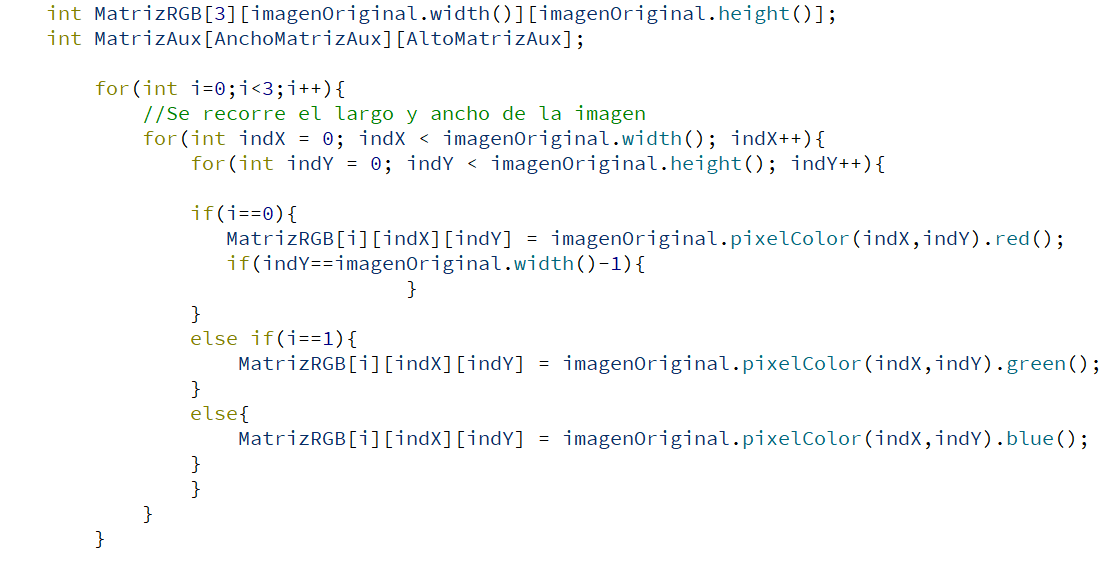
\includegraphics[width=15cm]{moduloMatrizRGB.png}
\centering
\caption{Matriz RGB}
\label{fig:matrizRGB}
\end{figure}

\item Después de tener las matrices de intensidad rojo, verde y azul guardadas en la metriz tridimensional MatrizRGB, procedemos a hacer el submuestreo de cada una de ellas, esto se logrará utilizando un while y un contador que se ocuparán de pasar por las tres matrices. Luego, a cada una de ellas se le irán sacando unas matrices auxiliares, las cuales tendrán un ancho y un largo de el largo y el ancho de las matrices originales dividido entre 16, que es el número de LEDs disponibles para la representación en Tinkercad.

\begin{figure}[h]
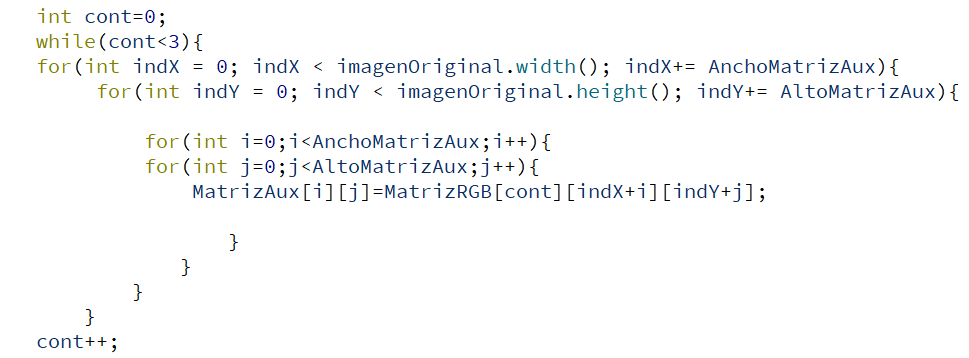
\includegraphics[width=15cm]{matrizaux.png}
\centering
\caption{Matriz auxiliar.}
\label{fig:matrizaux}
\end{figure}

\item Cada que se añade un elemento a la matriz auxiliar, este mismo elemento va sumándose con los demás elementos de la misma matriz para luego sacarle el promedio dividiendo entre la multiplicación del ancho por el alto de la matriz auxiliar. Este promedio calculado se va guardando en un arreglo llamado 'promedios' de tamaño 256.

\begin{figure}[h]
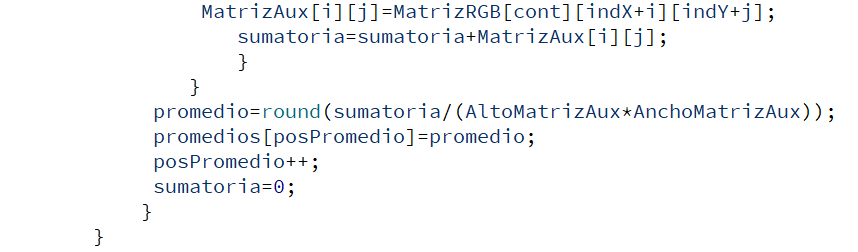
\includegraphics[width=15cm]{promedio.png}
\centering
\caption{Cálculo del promedio.}
\label{fig:promedio}
\end{figure}

\item Se recorre newMATRIZ que es la matriz obtenida por medio de promedios de la matriz original para convertirla a tamaño de 16x16, y se va rellenando haciendo uso del arreglo 'promedios', que iniciará en cero e irá aumentando de uno en uno hasta acabar el arreglo de tamaño 256.

En esta misma parte del código se escribe el archivo de texto llamado 'RGBbandera.txt', el cual contendrá la información de las tres matrices de intensidad necesarias para la simulación de Tinkercad.

\begin{figure}[h]
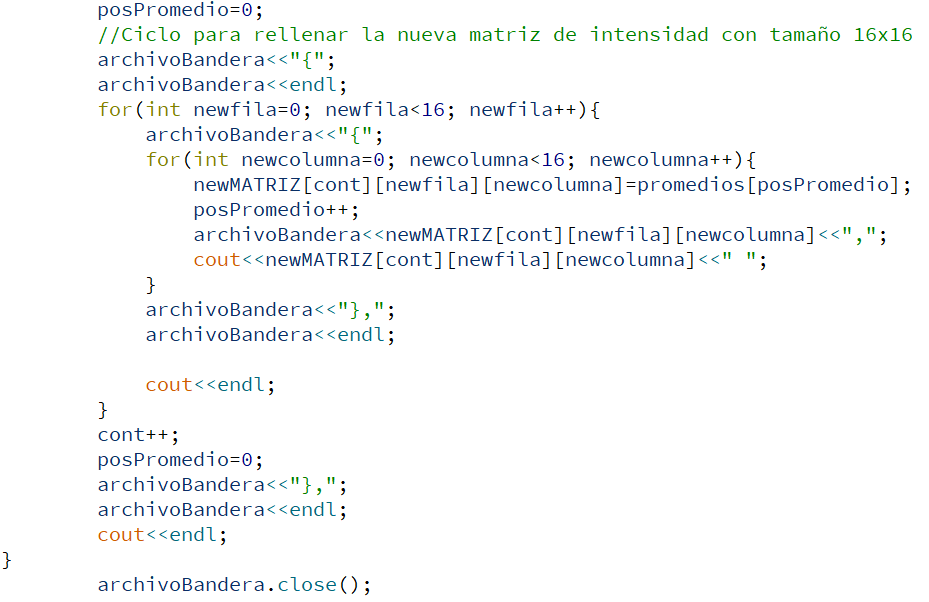
\includegraphics[width=13cm]{newmatriz.png}
\centering
\caption{Nueva matriz 16x16}
\label{fig:nuevamatriz}
\end{figure}

\end{enumerate}

\newpage
\section{Estructura del circuito} \label{circuito}

\begin{figure}[h]
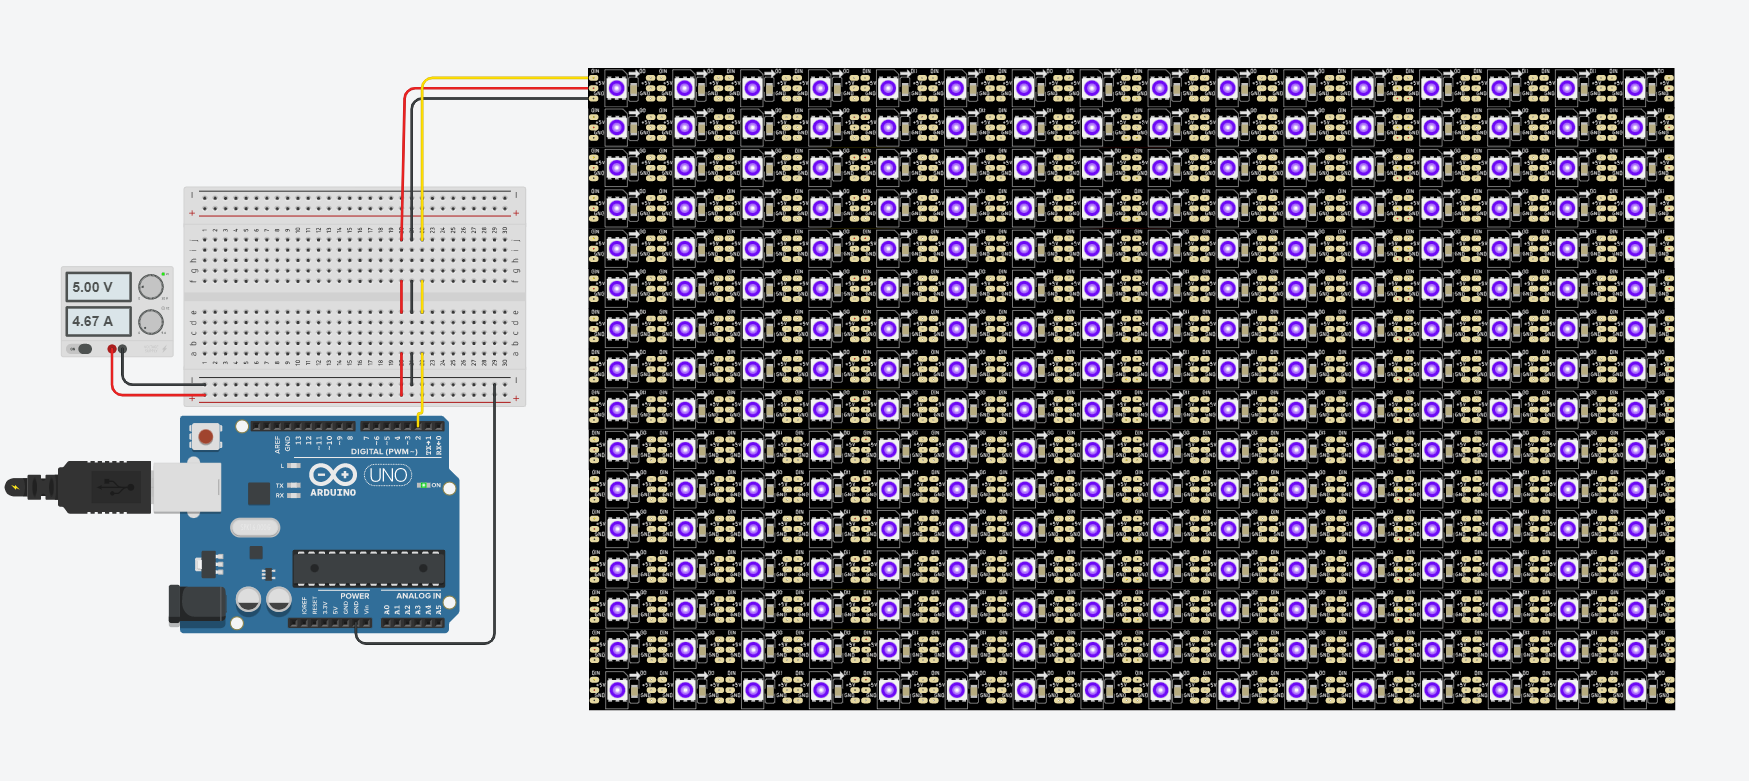
\includegraphics[width=15cm]{LEDs16x16.png}
\centering
\caption{Montaje de la matriz de LEDs de 16x16}
\label{fig:punto1}
\end{figure}

\newpage
\section{Problemas presentados} \label{problemas}
El principal problema presentado fue el encontrar una forma de reducir o amplificar el tamaño de las imágenes a 16x16, que es el tamaño decidido para representar las imágenes mediante las tiras de Neo Pixeles.


\end{document}
